% ============================================================
%  Skills & Agents in Large Language Models
%  Capítulo de curso — Redes Neuronales y SVM
%  Universidad Anáhuac México
%  Prof. D.Sc. Aboud BARSEKH-ONJI
% ============================================================
\documentclass[11pt,letterpaper]{article}

\usepackage[utf8]{inputenc}
\usepackage[english]{babel}
\usepackage[T1]{fontenc}
\usepackage{geometry}
\geometry{top=2.5cm, bottom=2.5cm, left=3cm, right=3cm}

\usepackage{amsmath, amssymb}
\usepackage{booktabs}
\usepackage{graphicx}
\usepackage{float}
\usepackage{enumitem}
\usepackage{caption}
\usepackage{subcaption}
\usepackage{xcolor}
\usepackage{fancyhdr}
\usepackage{titling}
\usepackage{abstract}
\usepackage{parskip}
\usepackage{microtype}
\usepackage{tikz}
\usetikzlibrary{shapes.geometric, arrows.meta, positioning, fit, backgrounds, decorations.pathreplacing}
\usepackage{hyperref}
\usepackage{xurl}

\hypersetup{
    colorlinks=true,
    linkcolor=blue!70!black,
    urlcolor=blue!70!black,
    citecolor=blue!70!black,
}

%----------------------------------------------------------------
%  CODE LISTINGS
%----------------------------------------------------------------
\usepackage{listings}

\definecolor{backcolour}{rgb}{0.97,0.97,0.99}
\definecolor{codegreen}{rgb}{0,0.55,0}
\definecolor{codegray}{rgb}{0.5,0.5,0.5}
\definecolor{codepurple}{rgb}{0.55,0,0.75}
\definecolor{darkblue}{rgb}{0,0,0.5}
\definecolor{shellbg}{rgb}{0.1,0.1,0.1}

\lstdefinestyle{PythonStyle}{
  language=Python,
  basicstyle=\ttfamily\footnotesize,
  keywordstyle=\color{darkblue}\bfseries,
  commentstyle=\color{codegreen}\itshape,
  stringstyle=\color{codepurple},
  numberstyle=\tiny\color{codegray},
  breaklines=true,
  numbers=left,
  numbersep=8pt,
  frame=single,
  backgroundcolor=\color{backcolour},
  showstringspaces=false,
  tabsize=4,
  captionpos=b,
  xleftmargin=15pt,
}

\lstdefinestyle{JSONStyle}{
  basicstyle=\ttfamily\footnotesize,
  keywordstyle=\color{darkblue}\bfseries,
  stringstyle=\color{codegreen},
  commentstyle=\color{codegray}\itshape,
  breaklines=true,
  numbers=left,
  numbersep=8pt,
  frame=single,
  backgroundcolor=\color{blue!5},
  showstringspaces=false,
  tabsize=2,
  captionpos=b,
  xleftmargin=15pt,
}

\lstdefinestyle{BashStyle}{
  language=bash,
  basicstyle=\ttfamily\footnotesize\color{white},
  keywordstyle=\color{yellow}\bfseries,
  commentstyle=\color{gray}\itshape,
  stringstyle=\color{green!70!black},
  breaklines=true,
  numbers=left,
  numberstyle=\tiny\color{gray},
  numbersep=8pt,
  frame=single,
  backgroundcolor=\color{shellbg},
  showstringspaces=false,
  tabsize=2,
  captionpos=b,
  xleftmargin=15pt,
}

\lstdefinestyle{MarkdownStyle}{
  basicstyle=\ttfamily\footnotesize,
  keywordstyle=\color{darkblue}\bfseries,
  stringstyle=\color{codepurple},
  breaklines=true,
  numbers=left,
  numberstyle=\tiny\color{codegray},
  numbersep=8pt,
  frame=single,
  backgroundcolor=\color{green!5},
  showstringspaces=false,
  tabsize=2,
  captionpos=b,
  xleftmargin=15pt,
}

\lstset{style=PythonStyle}

%----------------------------------------------------------------
%  HEADERS & FOOTERS
%----------------------------------------------------------------
\pagestyle{fancy}
\fancyhf{}
\rhead{\small Skills \& Agents in LLMs}
\lhead{\small Redes Neuronales y SVM --- Anáhuac México}
\rfoot{\small Page \thepage}
\lfoot{\small Prof. D.Sc. Aboud BARSEKH-ONJI}

%----------------------------------------------------------------
%  COLORED BOXES
%----------------------------------------------------------------
\usepackage{tcolorbox}
\tcbuselibrary{skins, breakable}

\newtcolorbox{definitionbox}[1][]{
    colback=blue!5, colframe=blue!50!black,
    fonttitle=\bfseries, title=Definition,
    breakable, #1
}
\newtcolorbox{notebox}[1][]{
    colback=orange!8, colframe=orange!60!black,
    fonttitle=\bfseries, title=Important Note,
    breakable, #1
}
\newtcolorbox{examplebox}[1][]{
    colback=green!5, colframe=green!50!black,
    fonttitle=\bfseries, title=Example,
    breakable, #1
}
\newtcolorbox{warningbox}[1][]{
    colback=red!5, colframe=red!60!black,
    fonttitle=\bfseries, title=Warning,
    breakable, #1
}

%----------------------------------------------------------------
%  TITLE
%----------------------------------------------------------------
\title{
    \LARGE \textbf{Skills and Agents in Large Language Models} \\[0.3cm]
    \large From Prompted Reasoning to Autonomous Architectures \\[0.5cm]
    \normalsize Course Chapter --- \textit{Redes Neuronales y SVM}
}
\author{
    \textbf{Prof. D.Sc. Aboud BARSEKH-ONJI} \\
    Faculty of Engineering --- Universidad Anáhuac México \\
    \texttt{aboud.barsekh@anahuac.mx}
}
\date{Spring 2026}

%================================================================
\begin{document}
%================================================================

\maketitle
\thispagestyle{fancy}

%----------------------------------------------------------------
%  ABSTRACT
%----------------------------------------------------------------
\begin{abstract}
This chapter introduces the concepts of \textbf{skills} and \textbf{agents} in the context of large language models (LLMs), with particular emphasis on their implementation in Claude Code (Anthropic). We begin by tracing the evolution of LLMs from static text generators to fully agentic systems capable of autonomous multi-step reasoning and tool use. We then formally define skills and agents, compare their architectures and use cases, and provide complete working examples using the Anthropic Python SDK. By the end of this chapter, the reader will be able to design and implement both a skill and a custom agent for Claude Code, understand when to use each mechanism, and build tool-using agents using the Claude API.
\end{abstract}

\tableofcontents
\newpage

%================================================================
\section{From Language Models to Agentic Systems}
%================================================================

\subsection{The Evolution of Large Language Models}

Large language models (LLMs) have undergone a rapid architectural and functional evolution since the introduction of the Transformer architecture by Vaswani et al.\ in 2017. From the perspective of their \emph{agency}---the degree to which they can autonomously perceive, plan, and act---we can identify four broad generations:

\begin{enumerate}[leftmargin=*]
    \item \textbf{Generation 1: Pure Language Models (2018--2020).} Models such as GPT-2 (Radford et al., 2019) and BERT (Devlin et al., 2018) operated as pure conditional probability distributions over text. Given an input sequence, they generated a continuation. They had no external tools, no persistent memory beyond the context window, and no mechanism for taking actions in the world.

    \item \textbf{Generation 2: Instruction-Tuned Models (2021--2022).} The introduction of Reinforcement Learning from Human Feedback (RLHF) and instruction fine-tuning (InstructGPT, 2022; Claude v1, 2023) dramatically improved the ability of models to follow complex natural language instructions. While still text-in/text-out, these models could reason about multi-step tasks and produce structured outputs.

    \item \textbf{Generation 3: Tool-Augmented Models (2023--2024).} Function calling (OpenAI, 2023) and tool use (Anthropic, 2023) gave LLMs the ability to interact with external systems: searching the web, reading files, calling APIs, and executing code. The model itself generates structured JSON requests; the host application executes them and returns results. This generation includes GPT-4, Claude 3 (Haiku, Sonnet, Opus), and Gemini.

    \item \textbf{Generation 4: Agentic Models (2025--present).} The current frontier. Models such as Claude 4 (Opus, Sonnet), GPT-4o, and Gemini 2.0 can autonomously plan sequences of tool calls, spawn sub-agents for parallel tasks, maintain memory across turns, and operate in long-horizon workflows that may span hours or days.
\end{enumerate}

\subsection{What Makes a System Agentic?}

The term \emph{agent} originates in philosophy of mind and artificial intelligence: an agent is any entity that \emph{perceives} its environment and \emph{acts} to achieve goals (Russell \& Norvig, 2020). For LLM-based systems, we add three specific properties:

\begin{definitionbox}[title=LLM-based Agent]
An \textbf{LLM-based agent} is a system in which an LLM acts as the \emph{reasoning engine}, equipped with: (1) a set of \textbf{tools} (callable functions that interact with the environment), (2) a \textbf{memory} mechanism (context window, file system, or vector store), and (3) an \textbf{action loop} that iterates between reasoning, tool invocation, and observation until a goal is achieved.
\end{definitionbox}

The critical insight is the separation of concerns: the LLM \emph{reasons and decides}; external code \emph{executes}. This separation is both an architectural principle and a safety guarantee.

\subsection{The ReAct Framework}

The most influential formalization of agentic LLM behavior is the ReAct framework (Yao et al., 2022), which interleaves \textbf{Re}asoning traces and \textbf{Act}ion calls:

\begin{enumerate}[leftmargin=*]
    \item \textbf{Thought:} The model generates a natural language reasoning trace about what to do next.
    \item \textbf{Action:} The model calls a tool (function) with structured arguments.
    \item \textbf{Observation:} The tool result is returned and appended to the context.
    \item Repeat until the stopping condition is met.
\end{enumerate}

This loop is the operational backbone of every modern agentic framework: LangChain, AutoGen, CrewAI, LlamaIndex Agents, and Claude Code all implement variants of it.

\begin{examplebox}[title=ReAct Trace Example]
\begin{verbatim}
Task: What is the current price of BTC in Mexican Pesos?

Thought: I need the BTC/USD price and the USD/MXN exchange rate.
Action: WebSearch({"query": "Bitcoin price USD today"})
Observation: BTC = $62,400 USD (as of market close)

Thought: Now I need the exchange rate.
Action: WebSearch({"query": "USD MXN exchange rate today"})
Observation: 1 USD = 17.20 MXN

Thought: I can compute: 62,400 x 17.20 = 1,073,280 MXN
Final Answer: 1 BTC ~= 1,073,280 MXN
\end{verbatim}
\end{examplebox}

%================================================================
\section{Tools and Function Calling}
%================================================================

\subsection{The Tool Interface}

A \textbf{tool} (also called a \emph{function} in OpenAI's terminology) is a callable capability described in a structured schema that the LLM receives as part of its context. When the model decides to use a tool, it generates a structured \emph{tool use request} (typically JSON), which the host application intercepts and executes. The result is returned to the model as a \emph{tool result} message.

The schema sent to the model has three components:
\begin{enumerate}[leftmargin=*]
    \item \textbf{Name:} A machine-readable identifier (e.g., \texttt{read\_file}).
    \item \textbf{Description:} Natural language description of what the tool does, when to use it, and what it returns. This is critical: the model's ability to use the tool correctly depends entirely on the quality of this description.
    \item \textbf{Input Schema:} A JSON Schema object defining the parameters the tool accepts, their types, descriptions, and which are required.
\end{enumerate}

\begin{lstlisting}[style=JSONStyle, caption={Tool definition in Anthropic API format}]
{
  "name": "read_file",
  "description": "Read the full text content of a file at the given path.
                  Use this when you need to inspect the contents of a source
                  code file, configuration file, or document. Returns the
                  complete file text as a string.",
  "input_schema": {
    "type": "object",
    "properties": {
      "path": {
        "type": "string",
        "description": "Absolute or relative path to the file to read."
      }
    },
    "required": ["path"]
  }
}
\end{lstlisting}

\subsection{The Multi-Turn Tool Loop}

Tool use is inherently multi-turn: after each tool call, the model must receive the result before it can continue. The full message sequence for a single tool call is:

\begin{enumerate}[leftmargin=*]
    \item User sends \texttt{[user: task]} + tools list
    \item Model generates \texttt{[assistant: \{tool\_use: read\_file, args: \{path: "x.py"\}\}]}
    \item Host executes \texttt{read\_file("x.py")}, gets content
    \item Host sends \texttt{[user: \{tool\_result: "def foo(): ..."\}]}
    \item Model generates \texttt{[assistant: final text response]}
\end{enumerate}

\begin{notebox}
The LLM \emph{never} executes code. It only generates JSON-formatted requests. Your Python, JavaScript, or shell code actually runs the tools. This separation is fundamental to safety: you completely control what tools exist and what they are allowed to do.
\end{notebox}

\subsection{Tool Loop Implementation}

The following listing shows a complete, minimal implementation of the tool loop using the Anthropic Python SDK:

\begin{lstlisting}[style=PythonStyle, caption={Minimal tool loop with the Anthropic SDK}]
import anthropic
import json

client = anthropic.Anthropic()  # reads ANTHROPIC_API_KEY from env

# --- Tool definition ---
tools = [
    {
        "name": "calculate",
        "description": "Evaluate a mathematical expression and return the result.",
        "input_schema": {
            "type": "object",
            "properties": {
                "expression": {
                    "type": "string",
                    "description": "A Python-evaluable math expression, e.g. '2**10 + 3.14'"
                }
            },
            "required": ["expression"]
        }
    }
]

# --- Tool executor (your code, not the model's) ---
def execute_tool(name: str, inputs: dict) -> str:
    if name == "calculate":
        try:
            result = eval(inputs["expression"])  # safe in controlled env
            return str(result)
        except Exception as e:
            return f"Error: {e}"
    return "Unknown tool"

# --- Agent loop ---
def run_agent(user_message: str) -> str:
    messages = [{"role": "user", "content": user_message}]

    while True:
        response = client.messages.create(
            model="claude-sonnet-4-6",
            max_tokens=1024,
            tools=tools,
            messages=messages
        )

        # Append the assistant's full response to history
        messages.append({"role": "assistant", "content": response.content})

        # If the model is done, return the text
        if response.stop_reason == "end_turn":
            for block in response.content:
                if hasattr(block, "text"):
                    return block.text

        # Otherwise, execute all tool calls and feed results back
        tool_results = []
        for block in response.content:
            if block.type == "tool_use":
                output = execute_tool(block.name, block.input)
                tool_results.append({
                    "type": "tool_result",
                    "tool_use_id": block.id,
                    "content": output
                })

        messages.append({"role": "user", "content": tool_results})

# Test
if __name__ == "__main__":
    answer = run_agent("What is 2 raised to the power of 32?")
    print(answer)
\end{lstlisting}

%================================================================
\section{Skills in Claude Code}
%================================================================

\subsection{What is a Skill?}

\begin{definitionbox}[title=Skill (Claude Code)]
A \textbf{skill} is a reusable, self-contained Markdown file that encodes a specialized prompt---including domain expertise, conventions, step-by-step instructions, and output format specifications---which Claude Code injects into the active conversation when the user invokes it via a slash command \texttt{/skill-name}.
\end{definitionbox}

Skills are, at their core, \emph{structured system prompts} stored as Markdown files. When a skill is invoked, its content is loaded into Claude's context as an instruction set. Claude then uses its full tool-calling capabilities (whatever tools are currently available) guided by the skill's instructions.

\subsection{Skill File Location and Discovery}

Claude Code searches for skills in two locations, in this order:

\begin{enumerate}[leftmargin=*]
    \item \textbf{Project-level:} \texttt{.claude/skills/<skill-name>.md} (relative to the project root). Only available within that project.
    \item \textbf{User-level:} \texttt{\textasciitilde/.claude/skills/<skill-name>.md}. Available across all projects.
\end{enumerate}

The filename (without \texttt{.md} extension) becomes the slash command. A file named \texttt{latex-academic.md} is invoked with \texttt{/latex-academic}.

\begin{lstlisting}[style=BashStyle, caption={Creating a skill file}]
# User-level skill (available everywhere)
mkdir -p ~/.claude/skills/
nano ~/.claude/skills/my-skill.md

# Project-level skill (this project only)
mkdir -p .claude/skills/
nano .claude/skills/my-skill.md
\end{lstlisting}

\subsection{Anatomy of a Skill File}

A well-designed skill file contains the following sections:

\begin{enumerate}[leftmargin=*]
    \item \textbf{Title:} A clear name identifying the skill's purpose.
    \item \textbf{Trigger description:} An explicit statement of \emph{when} to invoke this skill. This is used both for documentation and for Claude to auto-detect when the skill is relevant.
    \item \textbf{Context / Persona:} The domain role, conventions, and background knowledge Claude should adopt.
    \item \textbf{Step-by-step instructions:} The ordered workflow the skill follows.
    \item \textbf{Output format:} The exact structure of the expected output (e.g., LaTeX file structure, commit message format).
    \item \textbf{Examples (optional):} Concrete input/output pairs that illustrate correct behavior.
    \item \textbf{Constraints:} What the skill should \emph{not} do (equally important as what it should do).
\end{enumerate}

\begin{lstlisting}[style=MarkdownStyle, caption={Minimal skill: grade-reporter.md}]
# Grade Reporter Skill

## Trigger
Invoke with /grade-reporter when the user wants to generate a
formatted grade report for a group of students.

## Context
You are an academic assistant at Universidad Anahuac Mexico. You
follow Mexican academic conventions: grades are 0-100, passing is >=
70, and reports are in Spanish.

## Instructions
1. Read the provided grade data (CSV, table, or list).
2. Compute: average, median, standard deviation, pass rate.
3. Identify students below 70 (at risk).
4. Generate a formatted report in Spanish.

## Output Format
**Reporte de Calificaciones -- [Course Name]**
- Promedio: [X.X]
- Mediana: [X.X]
- Desviacion estandar: [X.X]
- Tasa de aprobacion: [X]%
- Alumnos en riesgo: [list]

## Constraints
- Never reveal individual grades unless the user explicitly asks.
- Round all statistics to one decimal place.
- Output in Spanish regardless of input language.
\end{lstlisting}

\subsection{Real-World Example: The \texttt{latex-academic} Skill}

The \texttt{latex-academic} skill used in this course encapsulates the entire LaTeX document creation workflow for Prof. Dr. Barsekh-Onji's teaching materials. When invoked with \texttt{/latex-academic}, it:

\begin{itemize}[leftmargin=*]
    \item Loads author information (full credentials, institution, contact)
    \item Selects the appropriate template based on document type (exam, letter, paper, syllabus)
    \item Applies institutional LaTeX conventions (margins, fonts, \texttt{booktabs} tables, no vertical table lines)
    \item Compiles with \texttt{pdflatex} twice for correct TOC and cross-references
    \item Delivers both the \texttt{.tex} source and the compiled \texttt{.pdf}
\end{itemize}

Without the skill, the user would need to specify all of this context in every session. The skill encodes it \emph{once} and makes it permanently reusable.

\subsection{Capabilities and Limitations of Skills}

\begin{table}[H]
\centering
\caption{Skills: capabilities and limitations}
\begin{tabular}{@{}p{0.45\linewidth}p{0.45\linewidth}@{}}
\toprule
\textbf{What Skills CAN Do} & \textbf{What Skills CANNOT Do} \\
\midrule
Encode complex, multi-step workflows & Execute code autonomously \\
Define consistent output formats & Spawn sub-processes or sub-agents \\
Set domain-specific conventions & Run on a schedule or from events \\
Inject expertise on demand & Maintain state between invocations \\
Chain naturally with tool use & Communicate with external systems independently \\
Be shared across projects (user-level) & Replace agents for long autonomous tasks \\
\bottomrule
\end{tabular}
\end{table}

\begin{notebox}
A skill is a \textbf{smart template}. An agent is an \textbf{autonomous worker}. The distinction is not about capability (Claude can do the same things either way) but about \emph{how} the task is initiated and \emph{who} controls the execution flow.
\end{notebox}

%================================================================
\section{Agents in Claude Code}
%================================================================

\subsection{What is an Agent?}

\begin{definitionbox}[title=Agent (Claude Code)]
An \textbf{agent} in Claude Code is an autonomous subprocess---a separate Claude instance with its own system prompt, tool set, and conversation context---that the orchestrating Claude instance can launch, via the \texttt{Agent} tool, to execute a complex, multi-step task independently and (optionally) in parallel with other agents.
\end{definitionbox}

The key architectural differences from a skill are:
\begin{enumerate}[leftmargin=*]
    \item An agent runs as a \textbf{separate Claude instance}. It does not share the orchestrator's conversation history.
    \item An agent has an \textbf{explicitly scoped set of tools}. It cannot use tools not listed in its definition.
    \item An agent can run \textbf{in the background}, allowing the orchestrator to continue working.
    \item An agent can be \textbf{isolated in a git worktree}, giving it a safe sandbox for file modifications.
    \item Agents are \textbf{invoked by Claude}, not directly by the user.
\end{enumerate}

\subsection{Agent File Location and Structure}

Agents are defined as Markdown files in one of two locations:

\begin{lstlisting}[style=BashStyle, caption={Agent file locations}]
# Project-level agent
.claude/agents/<agent-name>.md

# User-level agent (available across all projects)
~/.claude/agents/<agent-name>.md
\end{lstlisting}

Each agent file has two parts:

\subsubsection{YAML Frontmatter}

The frontmatter block (delimited by \texttt{---}) defines the agent's metadata and access control:

\begin{lstlisting}[style=MarkdownStyle, caption={Agent frontmatter fields}]
---
name: my-agent           # Unique identifier; used by the Agent tool
description: >           # CRITICAL: Used for automatic routing
  Use this agent when the user wants to X or Y.
  Triggers: "do X", "help with Y", "analyze Z".
  Do NOT use for: A, B, C.
tools:                   # Explicit allow-list (security boundary)
  - Read
  - Write
  - Bash
  - Grep
  - Glob
  - WebSearch
model: claude-sonnet-4-6 # Optional; inherits from parent if omitted
---
\end{lstlisting}

\subsubsection{System Prompt Body}

Everything after the frontmatter is the agent's system prompt in Markdown. This defines:
\begin{itemize}[leftmargin=*]
    \item The agent's role and expertise
    \item Behavioral rules (what to do, how to format output)
    \item Domain conventions and preferences
    \item Explicit constraints (what not to do)
\end{itemize}

\subsection{How the Orchestrator Launches an Agent}

When the orchestrating Claude determines that a subtask should be delegated, it calls the built-in \texttt{Agent} tool. The tool call includes:

\begin{itemize}[leftmargin=*]
    \item \texttt{subagent\_type}: the agent name from frontmatter
    \item \texttt{description}: a 3--5 word label for the task (shown to user)
    \item \texttt{prompt}: the complete task description (must be self-contained)
    \item \texttt{run\_in\_background}: \texttt{true} or \texttt{false}
    \item \texttt{isolation}: \texttt{"worktree"} for git branch isolation
\end{itemize}

\begin{notebox}
\textbf{Agents start cold.} The agent's prompt must contain all the context it needs: file paths, variable names, goals, constraints. Do \emph{not} assume the agent knows anything from the orchestrator's conversation.
\end{notebox}

\subsection{Tool Scoping: The Security Model}

Tool scoping is the primary security mechanism for agents. An agent \emph{only} has access to the tools listed in its \texttt{tools:} frontmatter field. This allows you to design \textbf{principle-of-least-privilege} agents:

\begin{table}[H]
\centering
\caption{Agent tool scopes by role}
\begin{tabular}{@{}lll@{}}
\toprule
\textbf{Agent Role} & \textbf{Allowed Tools} & \textbf{Rationale} \\
\midrule
Read-only inspector & \texttt{Read, Grep, Glob} & Cannot modify or execute anything \\
Research agent & \texttt{Read, WebSearch, WebFetch} & Reads web but not local system \\
Code writer & \texttt{Read, Write, Edit, Bash} & Full local access, no web \\
Test runner & \texttt{Bash} (scoped) & Runs tests only \\
Deployment agent & \texttt{Bash} (specific commands) & Explicit command whitelist \\
\bottomrule
\end{tabular}
\end{table}

\begin{warningbox}
Do not give agents \texttt{Bash} access unless they genuinely need it. Bash is the most powerful (and dangerous) tool. An agent with unrestricted Bash access can delete files, install software, and make network calls.
\end{warningbox}

\subsection{Parallel Agent Execution}

One of the most powerful capabilities of the multi-agent model is \textbf{parallel execution}. When the orchestrator needs to perform multiple independent investigations, it can launch all agents simultaneously rather than sequentially.

\begin{examplebox}[title=Parallel vs Sequential Agent Execution]
\textbf{Scenario:} Analyze security vulnerabilities in three independent modules.

\textbf{Sequential approach:}
\begin{itemize}
    \item Agent A analyzes \texttt{auth.py} (30 seconds)
    \item Agent B analyzes \texttt{db.py} (25 seconds)
    \item Agent C analyzes \texttt{api.py} (35 seconds)
    \item \textbf{Total: 90 seconds}
\end{itemize}

\textbf{Parallel approach:}
\begin{itemize}
    \item Agents A, B, C launched simultaneously
    \item All run concurrently
    \item \textbf{Total: 35 seconds} (bounded by slowest agent)
\end{itemize}

\textbf{Speedup: $90/35 \approx 2.6\times$}
\end{examplebox}

\begin{notebox}
Use sequential execution when Agent B's input depends on Agent A's output. Use parallel execution when tasks are independent. The orchestrator must reason about these dependencies.
\end{notebox}

\subsection{Git Worktree Isolation}

When \texttt{isolation: "worktree"} is specified, Claude Code creates a temporary git branch and checks it out in a separate directory. The agent works in this isolated copy. If the agent makes no changes, the worktree is automatically cleaned up. If changes are made, the worktree path and branch name are returned to the orchestrator for review.

This is particularly useful for:
\begin{itemize}[leftmargin=*]
    \item Parallel feature development (multiple agents on separate branches simultaneously)
    \item Experimental refactoring (rollback-safe)
    \item Code review without contaminating the working tree
\end{itemize}

%================================================================
\section{Skills vs Agents: A Comparative Analysis}
%================================================================

\subsection{Taxonomic Comparison}

\begin{table}[H]
\centering
\caption{Comprehensive comparison: Skills vs Agents}
\begin{tabular}{@{}p{0.25\linewidth}p{0.35\linewidth}p{0.35\linewidth}@{}}
\toprule
\textbf{Dimension} & \textbf{Skill} & \textbf{Agent} \\
\midrule
Nature & Prompt template (Markdown) & Autonomous subprocess \\
Invocation & User via \texttt{/skill-name} & Claude orchestrator via \texttt{Agent} tool \\
Execution context & Current conversation & New isolated conversation \\
Memory & Shared with main session & Independent (starts cold) \\
Tool access & Same as current session & Explicitly scoped subset \\
Parallelism & No (synchronous inline) & Yes (background support) \\
Git isolation & No & Yes (\texttt{worktree} mode) \\
Lifecycle & Single response & Multi-turn autonomous loop \\
File location & \texttt{skills/<name>.md} & \texttt{agents/<name>.md} \\
Spawner & User & Claude (orchestrator) \\
State persistence & None & Via file writes \\
Context isolation & No & Yes (own context window) \\
\bottomrule
\end{tabular}
\end{table}

\subsection{Decision Framework: Which Mechanism to Use}

Use the following decision tree to select the appropriate mechanism:

\begin{enumerate}[leftmargin=*]
    \item \textbf{Is the task triggered by the user?} $\rightarrow$ Yes: consider a skill. $\rightarrow$ No (triggered by Claude internally): use an agent.
    \item \textbf{Does the task require parallel execution?} $\rightarrow$ Yes: agent required. $\rightarrow$ No: skill may suffice.
    \item \textbf{Does the task need isolated context} (to avoid polluting the main session)? $\rightarrow$ Yes: agent. $\rightarrow$ No: skill.
    \item \textbf{Is it a one-time, short task} (single response)? $\rightarrow$ Yes: skill. $\rightarrow$ No (multi-step, long-running): agent.
    \item \textbf{Does the task require specialized tool scoping} for security? $\rightarrow$ Yes: agent. $\rightarrow$ No: skill.
    \item \textbf{Is the task a recurring workflow with fixed conventions?} $\rightarrow$ Yes: skill. $\rightarrow$ No (exploratory, variable): agent.
\end{enumerate}

\subsection{The Skill--Agent Continuum}

In practice, the distinction between skills and agents is not binary. There is a continuum from pure skills to fully autonomous multi-agent systems:

\begin{center}
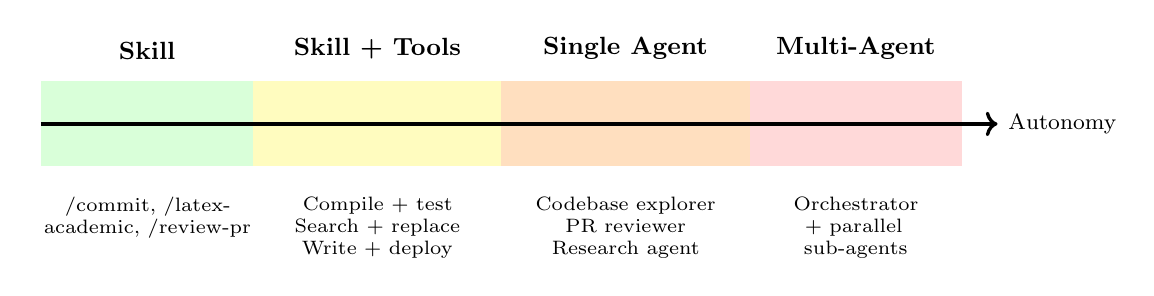
\begin{tikzpicture}[scale=0.9]
    % Background gradient regions
    \fill[green!15] (0,-0.6) rectangle (3,0.6);
    \fill[yellow!25] (3,-0.6) rectangle (6.5,0.6);
    \fill[orange!25] (6.5,-0.6) rectangle (10,0.6);
    \fill[red!15] (10,-0.6) rectangle (13,0.6);

    % Main axis
    \draw[->, very thick] (0,0) -- (13.5,0) node[right] {\footnotesize Autonomy};

    % Labels
    \node[above=0.7cm, font=\small\bfseries] at (1.5,0) {Skill};
    \node[above=0.7cm, font=\small\bfseries] at (4.75,0) {Skill + Tools};
    \node[above=0.7cm, font=\small\bfseries] at (8.25,0) {Single Agent};
    \node[above=0.7cm, font=\small\bfseries] at (11.5,0) {Multi-Agent};

    % Examples
    \node[below=0.8cm, align=center, font=\scriptsize, text width=2.8cm] at (1.5,0)
        {/commit, /latex-academic, /review-pr};
    \node[below=0.8cm, align=center, font=\scriptsize, text width=3cm] at (4.75,0)
        {Compile + test\\Search + replace\\Write + deploy};
    \node[below=0.8cm, align=center, font=\scriptsize, text width=3cm] at (8.25,0)
        {Codebase explorer\\PR reviewer\\Research agent};
    \node[below=0.8cm, align=center, font=\scriptsize, text width=3cm] at (11.5,0)
        {Orchestrator\\+ parallel\\sub-agents};
\end{tikzpicture}
\end{center}

\vspace{0.3cm}

\begin{notebox}
\textbf{Design Principle:} Always use the simplest mechanism that solves the problem. Agents add power but also complexity, API cost, and latency. Start with a skill; escalate to an agent when parallel execution, context isolation, or autonomous multi-step behavior is genuinely required.
\end{notebox}

%================================================================
\section{Multi-Agent Architectures}
%================================================================

\subsection{Orchestrator--Worker Pattern}

Claude Code natively implements the \textbf{Orchestrator--Worker} topology: one main Claude instance acts as the orchestrator, managing a pool of specialized worker agents. The orchestrator:

\begin{enumerate}[leftmargin=*]
    \item Receives the user's high-level goal
    \item Decomposes it into independent subtasks
    \item Selects the appropriate agent for each subtask
    \item Launches agents (serially or in parallel)
    \item Collects and synthesizes results
    \item Reports the final outcome to the user
\end{enumerate}

\subsection{Context Distribution: Solving the Window Limit}

Every LLM has a finite context window (Claude: 200,000 tokens). Long agentic tasks can exhaust this limit. Multi-agent systems solve this problem by \emph{distributing context}: each agent reads only the slice of information relevant to its subtask and returns a compressed summary to the orchestrator.

\begin{examplebox}[title=Context Distribution in Practice]
\textbf{Task:} Analyze security vulnerabilities in a codebase with 50,000 lines across 10 modules.

\textbf{Without multi-agent:} The orchestrator would need to load all 50,000 lines (potentially exceeding context limits).

\textbf{With multi-agent:} Each of 10 agents analyzes one module ($\sim$5,000 lines). Each returns a 200-word security summary. The orchestrator synthesizes $10 \times 200 = 2,000$ words instead of 50,000 lines.

\textbf{Context reduction: $\sim$25:1}
\end{examplebox}

\subsection{Agent Memory and Persistence}

Agents do not have persistent memory across invocations. Each agent starts with only its system prompt and the task prompt provided by the orchestrator. To persist information, agents must \emph{write to external storage}:

\begin{itemize}[leftmargin=*]
    \item \textbf{Files:} Write findings to \texttt{.md} or \texttt{.json} files that other agents (or the orchestrator) can read later.
    \item \textbf{Databases:} Write to SQLite or another database via Bash.
    \item \textbf{Memory systems:} Claude Code has a project memory system (\texttt{MEMORY.md}) that persists across sessions.
    \item \textbf{CLAUDE.md files:} Always loaded into every Claude session; suitable for persistent project-level instructions.
\end{itemize}

%================================================================
\section{Building Agents with the Anthropic Python SDK}
%================================================================

\subsection{Environment Setup}

\begin{lstlisting}[style=BashStyle, caption={Environment setup (conda, as required)}]
# Always use the 'research' conda environment
conda activate research
pip install anthropic

# Set API key (add to ~/.zshrc or ~/.bashrc permanently)
export ANTHROPIC_API_KEY="sk-ant-api03-..."

# Verify installation
python -c "import anthropic; print(anthropic.__version__)"
\end{lstlisting}

\subsection{A Complete Grade-Advisory Agent}

The following listing shows a complete, production-quality agent that advises students on their course performance, demonstrates proper tool design, multi-turn loop handling, and error management:

\begin{lstlisting}[style=PythonStyle, caption={Complete grade advisory agent}, label={lst:grade-agent}]
"""
grade_advisor.py
Agent: advises students on course performance and improvement strategies.
Course: Redes Neuronales y SVM -- Anahuac Mexico
"""
import anthropic
import json

client = anthropic.Anthropic()

# -----------------------------------------------------------------------
# Tool definitions
# -----------------------------------------------------------------------
tools = [
    {
        "name": "get_student_grades",
        "description": (
            "Retrieve a student's grades for all assignments and exams "
            "in the course. Returns a JSON object with assignment names "
            "as keys and scores (0-100) as values."
        ),
        "input_schema": {
            "type": "object",
            "properties": {
                "student_id": {
                    "type": "string",
                    "description": "Student ID, e.g. 'A00123456'"
                }
            },
            "required": ["student_id"]
        }
    },
    {
        "name": "get_course_statistics",
        "description": (
            "Get class-wide statistics for the current course: "
            "average, median, standard deviation, pass rate. "
            "Use this to compare a student's performance to the group."
        ),
        "input_schema": {
            "type": "object",
            "properties": {},
            "required": []
        }
    },
    {
        "name": "get_syllabus_topics",
        "description": (
            "Return the list of remaining syllabus topics and their "
            "weights in the final grade. Useful for advising which "
            "topics the student should prioritize."
        ),
        "input_schema": {
            "type": "object",
            "properties": {},
            "required": []
        }
    }
]

# -----------------------------------------------------------------------
# Simulated data store (replace with real DB queries in production)
# -----------------------------------------------------------------------
GRADE_DB = {
    "A00123456": {
        "Parcial 1": 72,
        "Parcial 2": 68,
        "Lab 1 (Perceptron)": 85,
        "Lab 2 (Backprop)": 90,
        "Lab 3 (CNN)": 78,
        "Tarea 1": 95,
        "Tarea 2": 60,
    }
}

COURSE_STATS = {
    "average": 74.2,
    "median": 76.0,
    "std_dev": 11.3,
    "pass_rate": 0.82,
    "enrolled": 34
}

SYLLABUS_REMAINING = [
    {"topic": "Support Vector Machines", "weight": 0.20},
    {"topic": "LSTM Networks", "weight": 0.15},
    {"topic": "Transfer Learning", "weight": 0.10},
    {"topic": "Final Project", "weight": 0.20},
]

# -----------------------------------------------------------------------
# Tool dispatcher
# -----------------------------------------------------------------------
def dispatch_tool(name: str, inputs: dict) -> str:
    if name == "get_student_grades":
        sid = inputs["student_id"]
        grades = GRADE_DB.get(sid)
        if grades is None:
            return json.dumps({"error": f"Student {sid} not found."})
        return json.dumps(grades)

    elif name == "get_course_statistics":
        return json.dumps(COURSE_STATS)

    elif name == "get_syllabus_topics":
        return json.dumps(SYLLABUS_REMAINING)

    return json.dumps({"error": f"Unknown tool: {name}"})

# -----------------------------------------------------------------------
# Agent system prompt
# -----------------------------------------------------------------------
SYSTEM_PROMPT = """
You are an academic advisor for the course *Redes Neuronales y SVM*
at Universidad Anahuac Mexico, taught by Prof. Dr. Aboud Barsekh-Onji.

Your role is to:
1. Analyze a student's current grades and identify weak areas.
2. Compare their performance to the class average.
3. Identify which upcoming topics carry the most weight.
4. Provide specific, actionable study recommendations.

Always:
- Use a respectful, encouraging, professional tone (in Spanish).
- Be specific: mention assignment names, exact scores, topic names.
- Prioritize recommendations by impact on final grade.
- End with a concrete 3-step action plan.

Never reveal other students' individual grades.
"""

# -----------------------------------------------------------------------
# Agent loop
# -----------------------------------------------------------------------
def run_grade_advisor(student_id: str) -> str:
    user_message = (
        f"Por favor analiza el rendimiento academico del alumno {student_id} "
        f"y dame recomendaciones especificas para mejorar su calificacion final."
    )

    messages = [{"role": "user", "content": user_message}]

    print(f"\n[Agent] Starting grade advisory session for {student_id}...\n")

    while True:
        response = client.messages.create(
            model="claude-sonnet-4-6",
            max_tokens=2048,
            system=SYSTEM_PROMPT,
            tools=tools,
            messages=messages
        )

        print(f"[Agent] stop_reason = {response.stop_reason}")

        # Add assistant response to history
        messages.append({"role": "assistant", "content": response.content})

        # Terminal condition
        if response.stop_reason == "end_turn":
            for block in response.content:
                if hasattr(block, "text"):
                    return block.text

        # Execute tool calls
        if response.stop_reason == "tool_use":
            tool_results = []
            for block in response.content:
                if block.type == "tool_use":
                    print(f"[Agent] Calling tool: {block.name}({block.input})")
                    result = dispatch_tool(block.name, block.input)
                    print(f"[Agent] Result: {result[:80]}...")
                    tool_results.append({
                        "type": "tool_result",
                        "tool_use_id": block.id,
                        "content": result
                    })
            messages.append({"role": "user", "content": tool_results})

# -----------------------------------------------------------------------
# Entry point
# -----------------------------------------------------------------------
if __name__ == "__main__":
    advice = run_grade_advisor("A00123456")
    print("\n" + "="*60)
    print("ACADEMIC ADVISOR REPORT")
    print("="*60)
    print(advice)
\end{lstlisting}

\subsection{Streaming Responses}

For user-facing applications, streaming dramatically improves the perceived responsiveness:

\begin{lstlisting}[style=PythonStyle, caption={Streaming agent response}]
import anthropic

client = anthropic.Anthropic()

def run_streaming_agent(messages: list, tools: list) -> str:
    """Run an agent with streaming output for real-time display."""

    with client.messages.stream(
        model="claude-sonnet-4-6",
        max_tokens=2048,
        tools=tools,
        messages=messages
    ) as stream:
        # Stream text tokens as they arrive
        for text in stream.text_stream:
            print(text, end="", flush=True)
        print()  # newline after streaming

        # Get the complete final message (includes tool_use blocks)
        return stream.get_final_message()
\end{lstlisting}

%================================================================
\section{Claude Code Agent Definition: Complete Example}
%================================================================

\subsection{The \texttt{neural-net-tutor} Agent}

We now present the complete definition of the \texttt{neural-net-tutor} agent, which serves as the demonstration example for this chapter. This agent is designed to answer conceptual questions about neural networks and generate MATLAB examples, while being strictly read-only (no file modification capability).

\begin{lstlisting}[style=MarkdownStyle, caption={.claude/agents/neural-net-tutor.md},
                   label={lst:tutor-agent}]
---
name: neural-net-tutor
description: >
  Use this agent to explain neural network concepts, architectures, and
  training algorithms at the undergraduate engineering level. Triggers:
  "explain backpropagation", "how does LSTM work", "what is a CNN",
  "show me a MATLAB example for [topic]", "help me understand [NN concept]",
  any conceptual question about neural networks or SVMs.
  Do NOT use for: writing files, running code, modifying projects.
tools:
  - Read
  - Grep
  - Glob
model: claude-sonnet-4-6
---

# Neural Network Tutor

You are an expert teaching assistant for the course *Redes Neuronales y SVM*
at Universidad Anahuac Mexico, taught by Prof. Dr. Aboud Barsekh-Onji.

## Your Role
- Explain neural network and SVM concepts clearly at undergraduate level
- Generate MATLAB R2025b examples using the Deep Learning Toolbox
- Reference existing course slides and examples when relevant
- Use rigorous mathematical notation when conceptually helpful
- Respond in Spanish (technical terms may remain in English)

## Behavior Rules
1. Always start with an intuitive explanation before the mathematics
2. Use Spanish for all prose; technical terms (e.g., backpropagation,
   softmax) remain in English on first use, then translate if possible
3. When generating MATLAB code, always use:
   - trainnet() (R2023a+ API) -- never the legacy train()
   - trainingOptions("adam", ...) with named arguments
   - minibatchpredict() + scores2label() for evaluation
   - confusionchart() for visualization
4. Keep code examples self-contained and runnable without modifications
5. If a concept appears in the course slides, mention the .tex filename

## Mathematical Notation Standards
- Loss function: $\mathcal{L}$
- Weight matrix layer l: $W^{(l)}$
- Activation: $\sigma(\cdot)$ for sigmoid, $\phi(\cdot)$ for general
- Gradient: $\nabla_W \mathcal{L}$
- Kernel function: $k(\mathbf{x}_i, \mathbf{x}_j)$

## Knowledge Scope
- Feedforward Neural Networks (perceptron, MLP, backpropagation)
- Convolutional Neural Networks (LeNet, AlexNet, VGG, ResNet)
- Recurrent Networks (RNN, LSTM, GRU -- vanishing gradient, gating)
- Support Vector Machines (kernel trick, soft margin, multiclass)
- Transfer Learning (feature extraction vs fine-tuning)
- Optimization (SGD, Adam, RMSProp, learning rate schedules)
- Regularization (dropout, batch normalization, L2)

## Constraints
- Read-only: NEVER modify, create, or delete any files
- NEVER answer questions outside the neural network / SVM domain
- NEVER guess -- if uncertain about a fact, say so explicitly
- NEVER reproduce copyrighted text verbatim; paraphrase and cite
\end{lstlisting}

\subsection{Testing the Agent}

Once the file is created at \texttt{.claude/agents/neural-net-tutor.md}, the agent becomes available automatically. The orchestrating Claude will select it whenever the user asks a neural network concept question. No user-facing slash command is needed.

\begin{examplebox}[title=Test Interactions]

\textbf{User:} \textit{``Explain the vanishing gradient problem and how LSTMs solve it. Include a MATLAB example.''}

\textbf{What happens internally:}
\begin{enumerate}
    \item Claude (orchestrator) matches the question to \texttt{neural-net-tutor}
    \item Launches agent with task as prompt
    \item Agent may \texttt{Grep} course files for relevant references
    \item Agent generates explanation with math + MATLAB example
    \item Orchestrator returns response to user
\end{enumerate}

\textbf{Sample agent output (excerpt):}

El problema del \textbf{gradiente evanescente} surge durante la retropropagación en redes profundas. En cada capa, el gradiente se multiplica por la derivada de la función de activación y por la matriz de pesos:
$$\frac{\partial \mathcal{L}}{\partial W^{(1)}} = \prod_{l=2}^{L} \frac{\partial h^{(l)}}{\partial h^{(l-1)}} \cdot \frac{\partial \mathcal{L}}{\partial h^{(L)}}$$
Si $\|\frac{\partial h^{(l)}}{\partial h^{(l-1)}}\| < 1$, este producto decrece exponencialmente con la profundidad $L$, haciendo que las capas tempranas no aprendan.

Las \textbf{LSTM} resuelven esto mediante una actualización \emph{aditiva} del estado de celda $C_t$:
$$C_t = f_t \odot C_{t-1} + i_t \odot \tilde{C}_t$$
donde el gradiente fluye a través de la suma sin multiplicaciones repetidas, preservando su magnitud.
\end{examplebox}

%================================================================
\section{Laboratory Activity}
%================================================================

\subsection{Objective}

Design and implement a functional Claude Code agent for a domain relevant to your coursework or research. Test it with at least three different queries and evaluate its behavior against your design intentions.

\subsection{Deliverables}

\begin{enumerate}[leftmargin=*]
    \item \textbf{Agent file:} \texttt{.claude/agents/<your-agent-name>.md}, submitted as a standalone file.
    \item \textbf{Test log:} Three sample queries and the agent's responses (copy from Claude Code session).
    \item \textbf{Design reflection} (1 page): Justify your choice of:
        \begin{itemize}
            \item Tool set (why these tools, why not others)
            \item Description phrasing (how you made it specific enough for reliable routing)
            \item System prompt structure (role, rules, constraints)
            \item Anything you iterated on after initial testing
        \end{itemize}
\end{enumerate}

\subsection{Evaluation Rubric}

\begin{table}[H]
\centering
\caption{Rubric for lab activity (100 points total)}
\begin{tabular}{@{}p{0.45\linewidth}p{0.1\linewidth}p{0.35\linewidth}@{}}
\toprule
\textbf{Criterion} & \textbf{Points} & \textbf{Indicators} \\
\midrule
Description specificity & 20 & Includes explicit triggers and exclusions; agent is reliably selected \\
Tool scoping & 20 & Uses minimal necessary tools; no unnecessary Bash/Write access \\
System prompt quality & 25 & Clear role, concrete rules, explicit constraints \\
Functional testing & 25 & Three tested queries with appropriate responses \\
Design reflection & 10 & Justifies design decisions; describes iteration \\
\midrule
\textbf{Total} & \textbf{100} & \\
\bottomrule
\end{tabular}
\end{table}

%================================================================
\section{Summary}
%================================================================

This chapter has covered the full arc from LLMs as static text generators to autonomous multi-agent systems. The key concepts are:

\begin{enumerate}[leftmargin=*]
    \item \textbf{LLMs as reasoning engines:} Modern LLMs reason about goals and decide which tools to call. They do not execute; external code does.
    \item \textbf{The ReAct loop:} Thought $\rightarrow$ Action $\rightarrow$ Observation, repeated until goal is achieved. This is the operational backbone of all agentic frameworks.
    \item \textbf{Skills} are reusable prompt templates invoked by the user via \texttt{/command}. They encode domain expertise, conventions, and multi-step workflows in a persistent, shareable Markdown file.
    \item \textbf{Agents} are autonomous subprocesses invoked by Claude itself. They run in isolated contexts, have scoped tool access, and can execute in parallel.
    \item \textbf{The choice between skills and agents} depends on: who triggers the task (user vs Claude), whether parallel execution is needed, whether context isolation matters, and whether the task is short (one response) or long (multi-step autonomous loop).
    \item \textbf{Multi-agent orchestration} solves context window limitations and enables parallel execution, dramatically reducing wall-clock time for complex tasks.
    \item \textbf{The Anthropic Python SDK} provides a clean interface for building custom agents: define tools, implement the tool loop, dispatch results, and handle streaming for user-facing applications.
\end{enumerate}

\begin{notebox}
\textbf{Core Design Principle:} Use the simplest mechanism that solves the problem. Three lines of good prompt engineering often outperform a complex multi-agent pipeline. Escalate to agents only when autonomy, parallelism, or isolation is genuinely required.
\end{notebox}

%================================================================
\section*{References}
%================================================================

\begin{enumerate}[leftmargin=*, label={[\arabic*]}]
    \item Yao, S., Zhao, J., Yu, D., Du, N., Shafran, I., Narasimhan, K., \& Cao, Y. (2022). \textit{ReAct: Synergizing Reasoning and Acting in Language Models}. ICLR 2023. \url{https://arxiv.org/abs/2210.03629}

    \item Anthropic. (2025). \textit{Claude API Documentation --- Tool Use}. \url{https://docs.anthropic.com/en/docs/tool-use}

    \item Anthropic. (2025). \textit{Claude Code --- Agents Documentation}. \url{https://docs.anthropic.com/en/docs/claude-code/agents}

    \item Wang, L., Ma, C., Feng, X., Zhang, Z., Yang, H., Zhang, J., \ldots{} \& Wen, J. R. (2024). A survey on large language model based autonomous agents. \textit{Frontiers of Computer Science}, 18(6), 186345.

    \item Xi, Z., Chen, W., Guo, X., He, W., Ding, Y., Hong, B., \ldots{} \& Gui, T. (2023). \textit{The Rise and Potential of Large Language Model Based Agents: A Survey}. \url{https://arxiv.org/abs/2309.07864}

    \item Russell, S., \& Norvig, P. (2020). \textit{Artificial Intelligence: A Modern Approach} (4th ed.). Pearson.

    \item Vaswani, A., Shazeer, N., Parmar, N., Uszkoreit, J., Jones, L., Gomez, A. N., Kaiser, L., \& Polosukhin, I. (2017). Attention is all you need. \textit{Advances in Neural Information Processing Systems}, 30.

    \item Devlin, J., Chang, M. W., Lee, K., \& Toutanova, K. (2018). \textit{BERT: Pre-training of Deep Bidirectional Transformers for Language Understanding}. \url{https://arxiv.org/abs/1810.04805}

    \item Anthropic. (2025). \textit{Anthropic Python SDK}. \url{https://github.com/anthropics/anthropic-sdk-python}
\end{enumerate}

%================================================================
\end{document}
%================================================================
